%-
% SPDX-License-Identifier: GPL-3.0-or-later
%
% This file is part of a firmware for Xling, a tamagotchi-like toy.
%
% Copyright (c) 2019 Dmitry Salychev
%
% Xling firmware is free software: you can redistribute it and/or modify
% it under the terms of the GNU General Public License as published by
% the Free Software Foundation, either version 3 of the License, or
% (at your option) any later version.
%
% Xling firmware is distributed in the hope that it will be useful,
% but WITHOUT ANY WARRANTY; without even the implied warranty of
% MERCHANTABILITY or FITNESS FOR A PARTICULAR PURPOSE.  See the
% GNU General Public License for more details.
%
% You should have received a copy of the GNU General Public License
% along with this program.  If not, see <https://www.gnu.org/licenses/>.

%
% LaTeX sources of the Xling User Manual.
%
\documentclass[11pt,a4paper,twoside]{report}

%
% Packages.
%
%\usepackage{showframe}
\usepackage[utf8]{inputenc}
\usepackage{geometry}
\usepackage{graphicx}
\usepackage{caption}
\usepackage{subcaption}
\usepackage{blindtext}
\usepackage{layout}
\usepackage{hyperref}
%\usepackage{mfirstuc}			% helps to make First Capital Letters.
\usepackage[nameinlink]{cleveref}	% helps to make Capitalized references.

%
% Page configuration.
%
% NOTE: See http://www.texdoc.net/texmf-dist/doc/latex/geometry/geometry.pdf
%       for details.
%
\geometry{
	includehead,	% head will be included into total body
	includefoot,	% foot will be included into total body
	inner=72pt,	% left margin (between paper and total body)
	outer=72pt,	% right margin (between paper and total body)
	top=50pt,	% top margin (between paper and total body)
	bottom=50pt,	% bottom margin (between paper and total body)
}

%
% Hyperlinks setup.
%
% NOTE: See https://en.wikibooks.org/wiki/LaTeX/Hyperlinks for details.
%
% NOTE: See https://sunsite.icm.edu.pl/pub/CTAN/macros/latex/contrib/
%	cleveref/cleveref.pdf for details.
%
\hypersetup{
	bookmarks=true,		% create PDF bookmarks/outline?
	hidelinks,		% hide links (removing color and border)
}

%
% Graphicx package setup.
%
\graphicspath{ {./images/} }

\renewcommand{\familydefault}{\sfdefault}
\everymath={\sf}

\title{Xling User Manual}
\author{Dmitry Salychev}
\setcounter{tocdepth}{2}

% -----------------------------------------------------------------------------
% Document
% -----------------------------------------------------------------------------
\begin{document}

\maketitle
\tableofcontents

\chapter*{Introduction}
Congratulations! It looks like you bought a kit to build Xling,
a tamagotchi-like toy, or decided to follow your own way to assemble and
program it from scratch. This manual will help you anyway. Chapters of the
document are placed in a logical order to make the device ready to be
programmed, tested and populated with your own firmware.
\\
\\
\textbf{\Cref{chap:safety}} should be read first in order to understand how to
build and use Xling safely and prevent any damage.
\textbf{\Cref{chap:assembling_device}} is a good place to start if you're
going to build the device from scratch and its
\textbf{\Cref{sec:board_from_prebuilt_kit}} will help you to finish the
pre-built Xling. \textbf{\Cref{chap:testing_device}}
will cover several topics about understanding your device is built correctly
and ready to be used.
\textbf{\Cref{chap:building_firmware}} explains how to get sources of the basic
Xling firmware\footnote{https://github.com/mcusim/Xling}, build it and upload
to the device.
\\
\\
Initially, Xling was meant to be a simple, but well made toy for my wife which
should be fun and particularly easy to made. And it turned out exactly as I
imagined with 8-bit AVR microcontroller, 128x64 OLED display and a battery
charging circuit. Its PCB design files and source code of the firmware are
distributed under open source licenses\footnote{CERN-OHL-W v2 and GNU GPLv3+
accordingly} which makes this toy a perfect candidate to study from hardware
and software point of view. You might find it even more interesting because
FreeRTOS, a well known and probably the most popular real-time operating system,
is used to power Xling.
\\
\\
Enjoy.
\\
\\
Regards\\
Dmitry Salychev\\
dsl@MCUSim.org

% -----------------------------------------------------------------------------
% Chapter: Safety.
% -----------------------------------------------------------------------------
\chapter{Safety}
\label{chap:safety}
Please, note that Xling is an open hardware DIY\footnote{do-it-yourself}
electronic toy which hasn't been certified against any electrical safety
standards. However, it doesn't mean that you should ignore rules which help
to prevent damage to your property or health.
\\
\\
Safety rules are:
\begin{enumerate}
	\item
	Do not try to assemble, repair or disassemble Xling yourself if you
	don't know how to work with laboratory equipment like soldering irons,
	hot air guns, desolderings tools, etc.
	\item
	Do not damage Xling or its parts. It carries a fragile OLED display
	which is made using glass. LiPo battery should not be damaged or
	disassembled.
	\item
	Do not try to change firmware of the device if you aren't sure that
	your changes won't break battery charging circuit\footnote{if in doubt,
	ask dsl@MCUSim.org} work.
	\item
	Xling doesn't have a protection against water or dust. You should be
	careful with using it outdoor.
\end{enumerate}

% -----------------------------------------------------------------------------
% Chapter: Assembling the device.
% -----------------------------------------------------------------------------
\chapter{Assembling the device}
\label{chap:assembling_device}
Xling has been designed to be a device easy to made. It means that almost
everything\footnote{except PCB itself, probably} can be done on your own.
For example, if you've a decent 3D printer and some experience printing things
from PETG, you'll be able to produce a case for Xling. If you've a good
soldering iron, a hot air gun, and an ability to solder components as small
as 0603, you'll be able to assemble PCB then.
\\
\\
The following sections are supposed to help you taking steps from gathering
components from the BOM and checking that you've all of the required tools and
equipment to assemble the board to several final steps to finish the board by
chosing and soldering a suitable LiPo battery in order to support an idea
behind this chapter which is to let you start from any point depending on
what you've at your hands.

\section{Overview of the Xling kit}
\label{sec:overview_of_the_kit}

\section{Starting from scratch}
\label{sec:board_from_scratch}
[ section under construction ]

\section{Assembling the board}
\label{sec:board_from_kit}
[ section under construction ]

\section{Finishing the board}
\label{sec:board_from_prebuilt_kit}
This section will guide you through a process of finishing the Xling PCB
to make it ready to be tested and placed into a 3D printed case. It is usually
a convenient way to get a toy ready in only a fraction of that amount of time
which might be necessary to build it from scratch.
\begin{figure}[h]
	\centering
	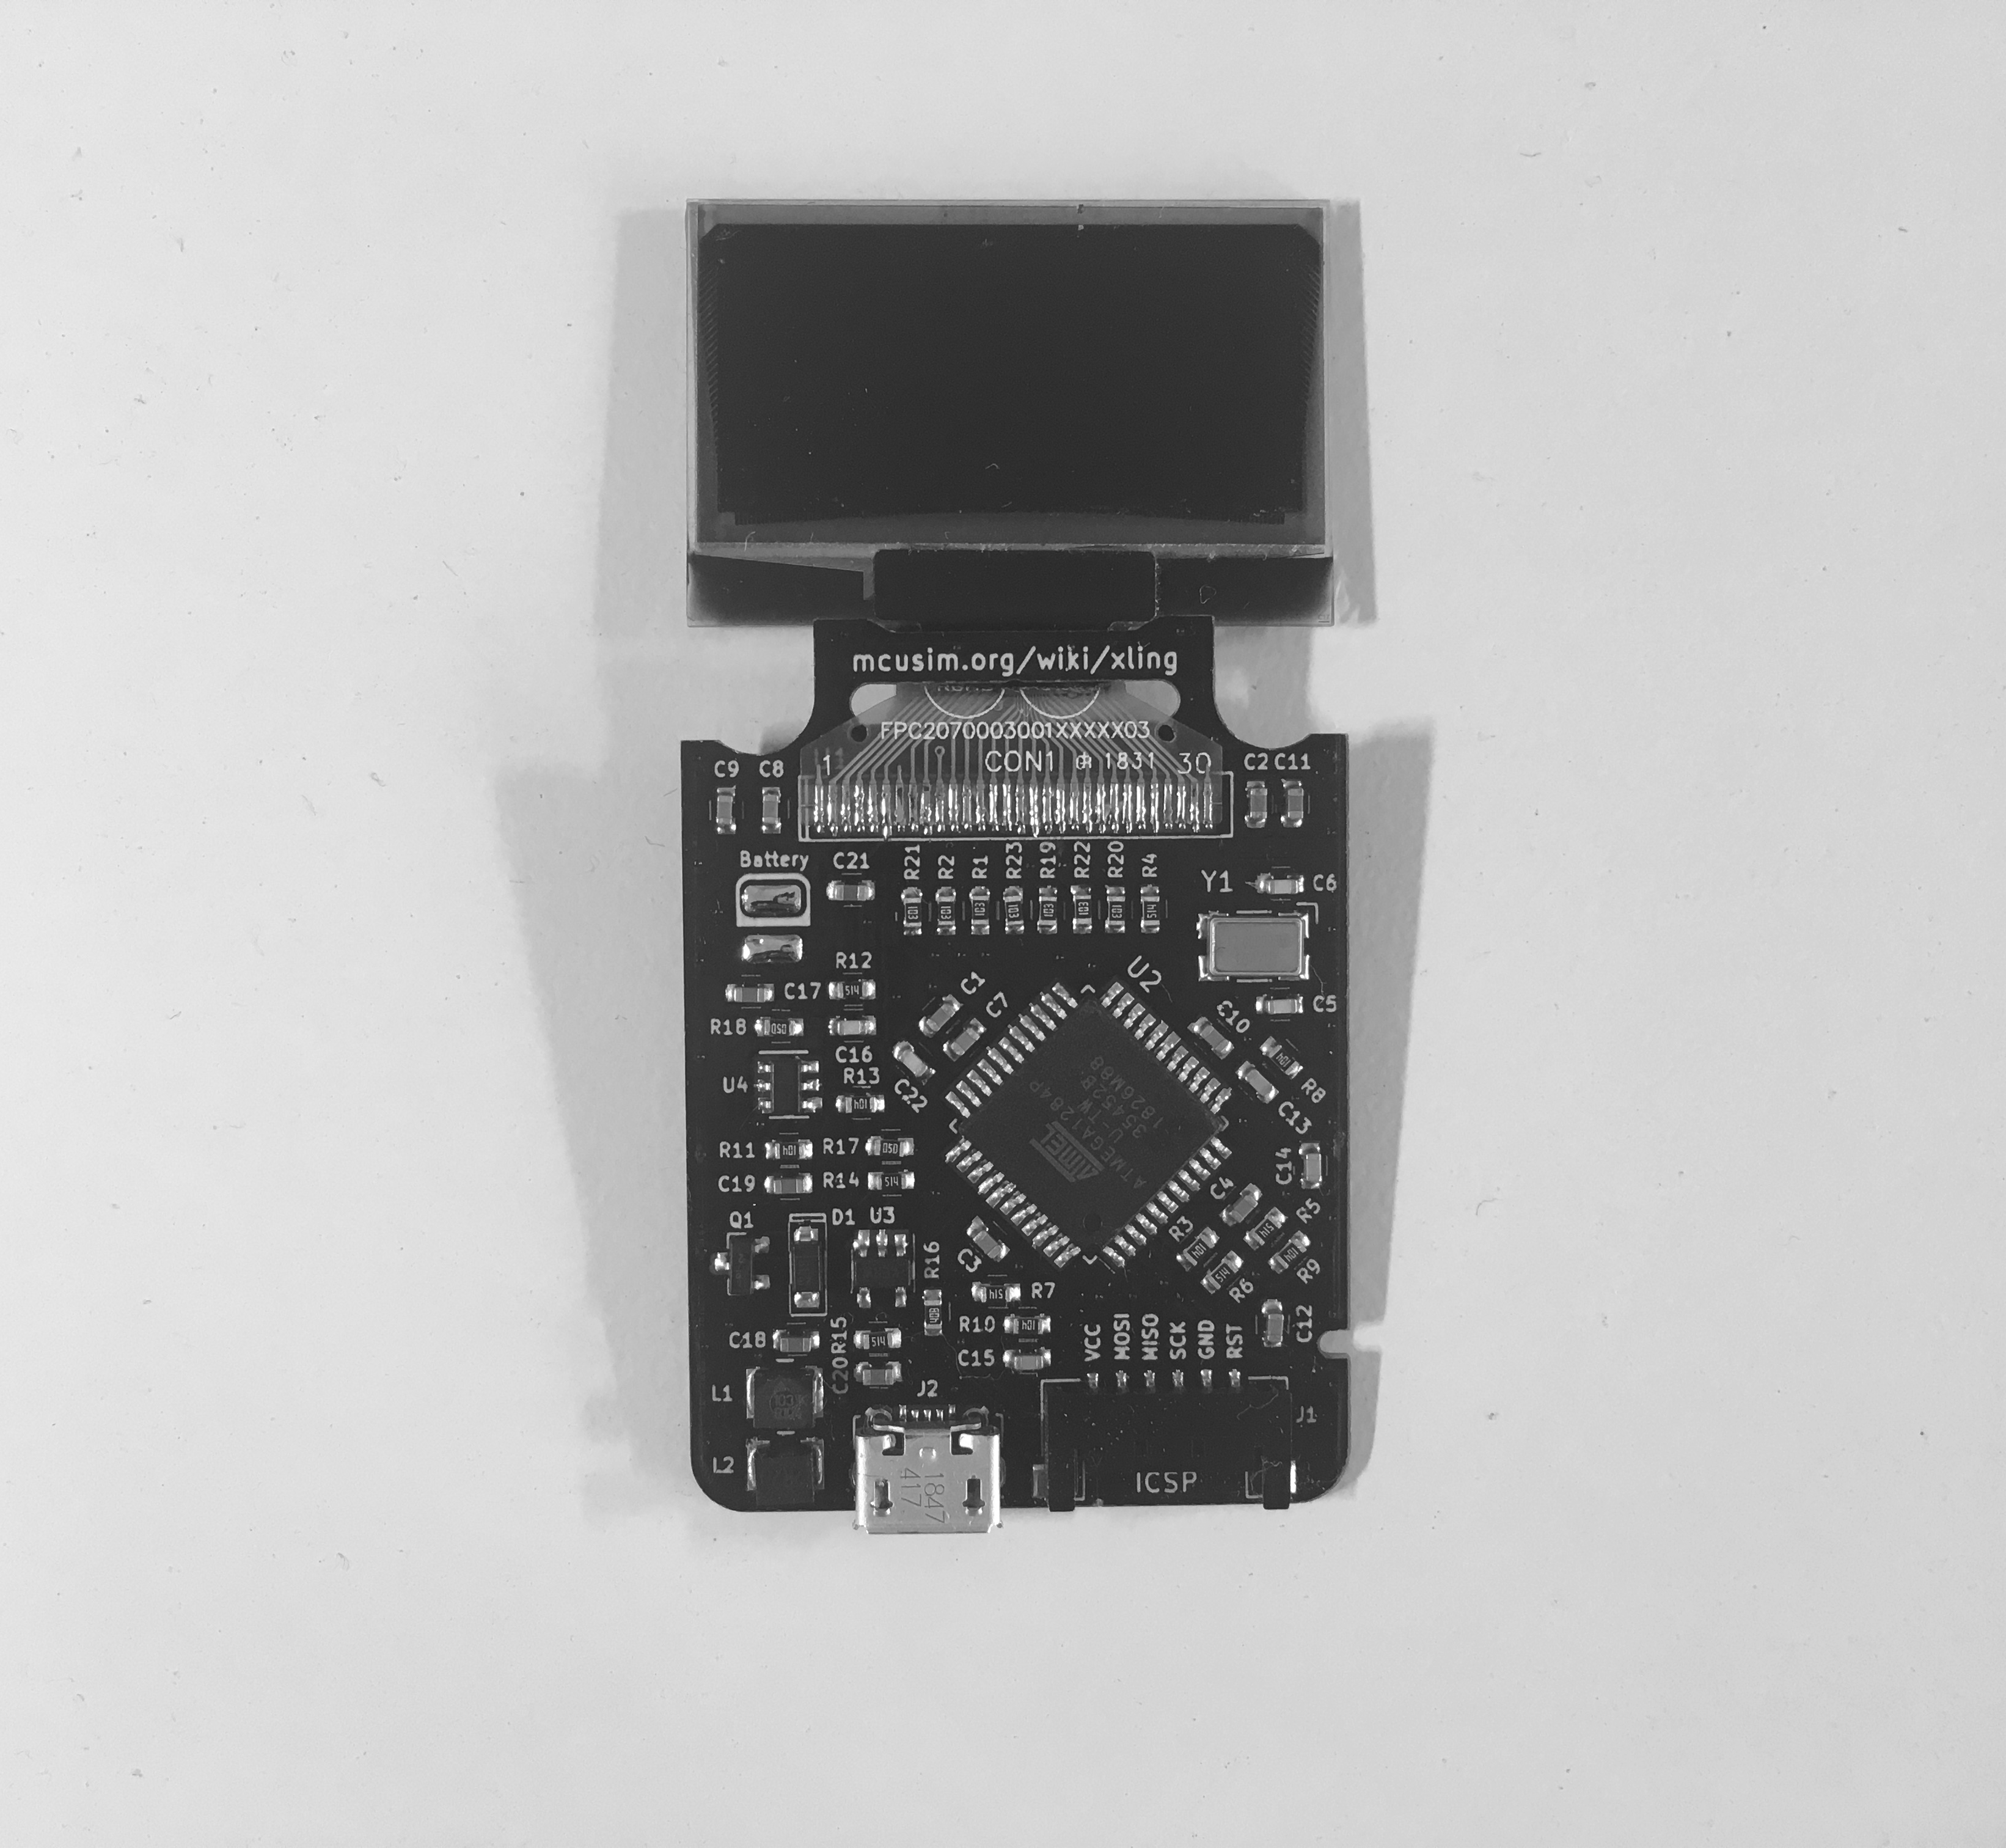
\includegraphics[height=9cm]{prebuilt_pcb_grayscale}
	\caption{Pre-built Xling PCB}
\end{figure}

% -----------------------------------------------------------------------------
% Chapter: Testing the device.
% -----------------------------------------------------------------------------
\chapter{Testing the device}
\label{chap:testing_device}
[ section under construction ]

% -----------------------------------------------------------------------------
% Chapter: Building firmware.
% -----------------------------------------------------------------------------
\chapter{Building and uploading firmware}
\label{chap:building_firmware}
[ section under construction ]

\end{document}
